

\chapter{Conclusion}

\label{chap:conclusion} 
\newcommand{\typetutor}{TypeTutor}

\graphicspath{{Figures/Conclusion}}
At the beginning of this thesis, we gave an overview of the landscape of programming languages, with a special interest in functional programming and static typing. We emphasized the critical role of type errors, noting how problematic type errors can hinder both the learning and the effective use of statically typed languages. Then, we explored various Haskell type-checking methods and their evolution, setting the stage for an in-depth discussion of our interventions, \chameleon{}, Goanna, and GeckoGraph, which are designed to deliver accurate and user-friendly error messages.

In this chapter, we review our contributions and discuss the future work that builds upon these initiatives. The planned future work encompasses what we consider a natural next step in tool design, integration with large language models (LLMs), and language availability. We provide detailed visions for how debugging type errors can be further improved using our acquired knowledge. We conclude our discussion by reaffirming our commitment to improving type errors, a core objective of this thesis, and reiterating the importance of this work within the broader field of programming language research.


\section{Contributions}

In this thesis, we present four key areas of contribution: a categorization of type errors, \chameleon{}, Goanna, and GeckoGraph. 

\subsection*{A categorization of type errors}


We have developed a categorization framework for type errors based on insights into how human programmers perceive them and theories from constraint satisfiability research. This framework helps identify three critical attributes of type errors, enhancing our understanding of strategic interventions to assist programmers in effectively resolving these errors.

\begin{itemize}
    \item {\textbf{Multi-step type errors} These errors involve a sequence of logical deductions, requiring programmers to look for multiple locations of the source code to forge a coherent reasoning chain. It is crucial to clearly present these locations and their interconnected relationships within the source code to streamline this reasoning process.}
    \item{\textbf{Multi-witness type errors}  These errors present an imbalance in the evidence, leading to two possible causes. Highlighting this discrepancy can guide programmers toward a more informed evaluation of the likely root causes, aiding in quicker resolution.}
    \item{\textbf{Multi-party type errors} These errors involve conflicts that present more than two potential possible types. They often indicate the coexistence of multiple underlying errors. Providing tools that can break down these errors into multiple type errors of simpler form allows programmers to tackle each error sequentially, leading to a simpler debugging workflow.}
\end{itemize}


Following this classification, we delved into the three main systems we developed in our research:\chameleon{} (see Chapter \ref{chap:chameleon}), Goanna (see Chapter \ref{chap:goanna}), and GeckoGraph (see Chapter \ref{chap:gecko-graph}). Each system is designed to tackle some different challenges associated with debugging type errors.

\subsection*{Explain Multi-step type errors and the chain of thought visualization}


We introduce \textbf{\chameleon{}}, an interactive Haskell type error debugging tool. \chameleon{} uses Minimal Unsatisfiable Subsets (MUS) as its core type error representation. Our work on \chameleon{} is based on the existing work on Chameleon \cite{Stuckey2003-pz, Wazny2006-ll}. The original Chameleon was developed as a command-line tool; its innovative approach of interactive debugging allows programmers to view different possible type error explanations and type assignments by issuing console commands.  We took the idea of an MUS-based Haskell debugging tool and interactive debugging techniques and provided a modern implementation with many advanced features. Notably, \chameleon{} enables programmers to explore the chain of reasoning behind type errors in step-by-step order. Additionally, \chameleon{} features an adaptive user interface, allowing programmers to tailor the information density of type errors according to their experience level.


We conducted three user studies to investigate the impacts of using debugging tools that support type error slicing and interactive type error exploration, some key features provided in \chameleon{}. Our findings reveal a notable improvement in debugging speed when employing the type error-slicing technique, particularly for complex tasks. Additionally, across the experience level, we observed a significant enhancement in debugging speed when programmers engaged with the interactive debugging features, suggesting that active exploration of type errors can positively impact the debugging process.

\subsection*{Resolve multi-witness and multi-party errors with Minimal Correction Subsets}

We contribute \textbf{Goanna}, a Haskell type error debugging tool that, like \chameleon{}, utilizes type error slicing to achieve comprehensive and user-friendly error localization.

Goanna sets itself apart by employing Minimal Correction Sets (MCS) to identify potential causes of type errors. It conducts an exhaustive analysis of all potential causes and corresponding actions required to resolve the type error. In addition, Goanna employs a set of heuristics to avoid an overwhelming list of suggestions. These heuristics filter out less useful suggestions and prioritize potential causes based on their likelihood, ensuring a more focused and effective debugging experience.


To assess the efficacy of MCS-based type error debugging strategies, we compiled a dataset of 86 Haskell programs sourced from various online discussions, embodying a wide range of type error scenarios. We evaluated the accuracy of Goanna in identifying and resolving type errors in comparison to traditional compiler tools. Our findings affirm that Goanna consistently provides more accurate error-cause identification compared to other tools. Further, our heuristics not only effectively narrow down the list of possible causes but also consistently include the real cause in its top recommendations. Lastly, although Goanna is slower than the conventional tools, it remains well within a range suitable for providing real-time feedback. 

\subsection*{Visualizing Types}

We introduce \textbf{GeckoGraph}, an innovative graphic notation system designed specifically for Haskell types. Unlike traditional type signatures, GeckoGraph utilizes a combination of colors, shapes, and symbols to highlight distinct type structures. GeckoGraph provides a clear visual representation for type-level features such as type classes, parametric type variables, and high-rank types. When programmers need to compare two types, a frequent requirement in resolving type errors, GeckoGraph provides strong visual grouping that is often able to underscore subtle differences, providing clear graphical distinctions.

We conducted a large-scale user study to evaluate the effectiveness of GeckoGraph in enhancing the traditional text-based approach to type signatures. The study was designed as an interactive puzzle game incorporating gamification elements to stimulate participation and engagement. In total,  721 programmers of all experience levels participated in the study. While the results showed that the use of GeckoGraph did not significantly impact the speed or overall success rate of solving problems, it proved significant in supporting beginners in solving harder tasks more successfully. Additionally, feedback collected through a qualitative post-study survey was positive, suggesting that GeckoGraph is intuitive, non-intrusive, and helpful.

\section{Future Work}

In this section, we present three promising directions stemming from our existing work. Firstly, drawing upon our prior experience of researching type debugging tools, we now sketch a novel debugging tool: \textit{TypeTutor}. We envision the interfaces and interactions within \textit{TypeTutor}, which have been shaped by insights from our existing tools and feedback from various user studies.

Secondly, we delve into the realm of rapid advancements in large language models (LLMs) and their evolving role in programming assistance, distinguishing them from conventional theory-based tools like \chameleon{} and Goanna. We explore the possibility of integrating traditional tools with LLMs to effectively capitalize on their unique strengths and address their weaknesses.

Lastly, we outline our plans to adapt our debugging tools for use in other programming languages, underscoring the potential advantages and challenges associated with this endeavor.

\subsection*{\typetutor: Question-Based Type Debugging}

By observing programmers tackle type error challenges in a series of user studies, we gained valuable insights into Haskell programmers' debugging habits and approaches toward challenging type errors. Armed with this understanding, we are inspired to envision a novel debugging tool named \textit{TypeTutor}. The core concept of \textit{TypeTutor} would be to map debugging tasks into a series of questions that programmers would naturally ask while also to help programmers break down high-level debugging questions into actionable, granular queries.

This style of programming is often referred to as ``natural programming environment'' \cite{Myers2004-fy}. Previous studies have underscored the benefits of employing a natural debugging interface, exemplified by tools such as Alice~\cite{Conway2000-nn} and WhyLine~\cite{Ko2009-uf}. However, existing research predominantly concentrates on debugging runtime errors, neglecting exploration into type-level debugging.  Leveraging our experience with \chameleon{}, Goanna, and GeckoGraph, we envision meaningful progress in this domain.


\subsubsection*{Why questions}

A fundamental aspect of debugging type errors involves asking questions such as "Why does the type error occur?" and "Why is the expected type \texttt{X}?" These "why" questions highlight gaps in understanding where a thorough explanation is in demand. \textit{TypeTutor} will intelligently address this by displaying all relevant "why" questions when a programmer hovers over an expression of interest. Upon selecting a question, \textit{TypeTutor} will promptly provide the corresponding detailed answer (Fig.~\ref{fig:why}).



\begin{figure}[hbt]
  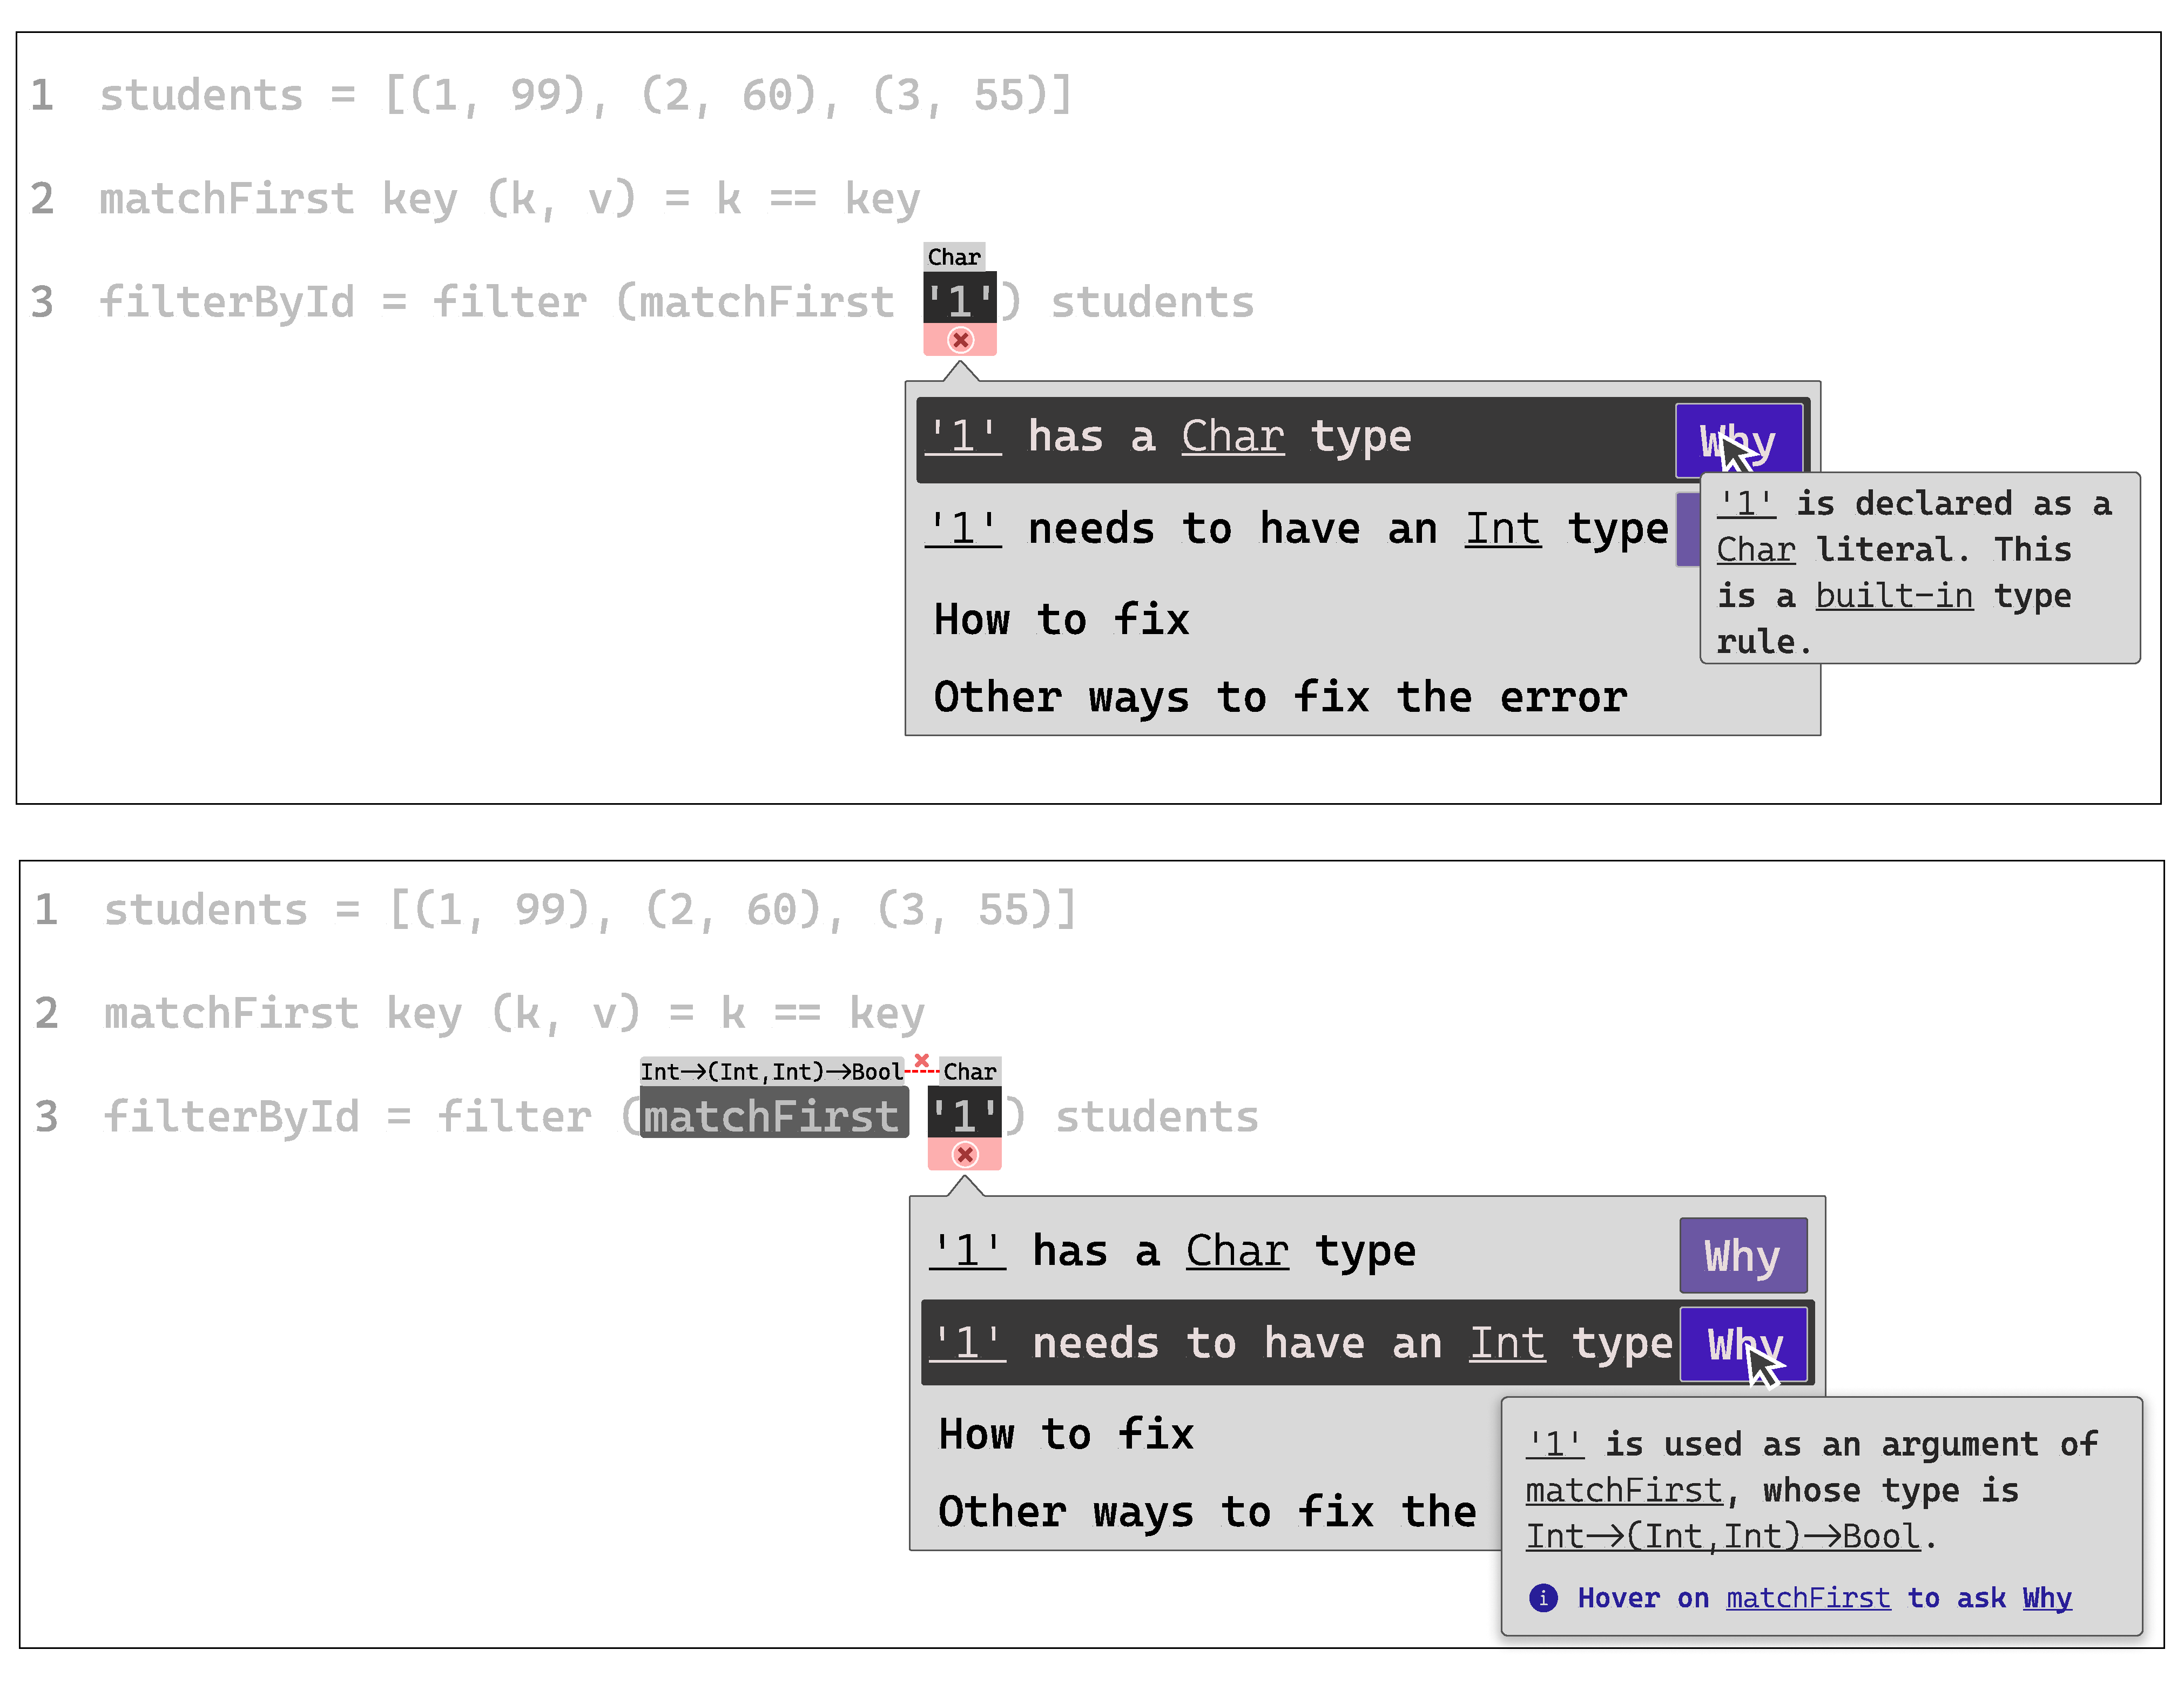
\includegraphics[width=\linewidth]{Why}
  \caption[An example of \textit{TypeTutor} providing explanation (`why' questions)]{
      \label{fig:why}
      The figure shows how \textit{TypeTutor} would provide programmers valid `why' questions to ask in a type error. When hovering on a location that is marked as a type error, \textit{TypeTutor} will identify an `expected' type (Top) and an `actual' type (Bottom). \textit{TypeTutor} would also prompt programmers to interrogate each branch to understand how these conclusions are drawn by hovering on the `Why' buttons. 
    }
\end{figure}



\subsubsection*{Follow-up questions}

In the context of debugging type errors, particularly multi-step type errors, it proves beneficial to enable programmers to incrementally uncover the underlying inference logic. \textit{TypeTutor} will support this process by allowing programmers to ask follow-up questions. Typically, these questions build upon the responses to earlier inquiries. Follow-up questions in \textit{TypeTutor} would facilitate tasks akin to the interactive debugging steps in \chameleon{}. However, unlike \chameleon{}, \textit{TypeTutor} would not need a separate interface for such a task. Instead, when a response includes the option for further inquiry, \textit{TypeTutor} would provide a follow-up hint at the end of the answer, encouraging programmers to continue tracing the root cause (Fig.~\ref{fig:follow-up}). This integrated approach would help maintain a streamlined user experience while enabling deep exploration of type errors.


\begin{figure}[hbt]
  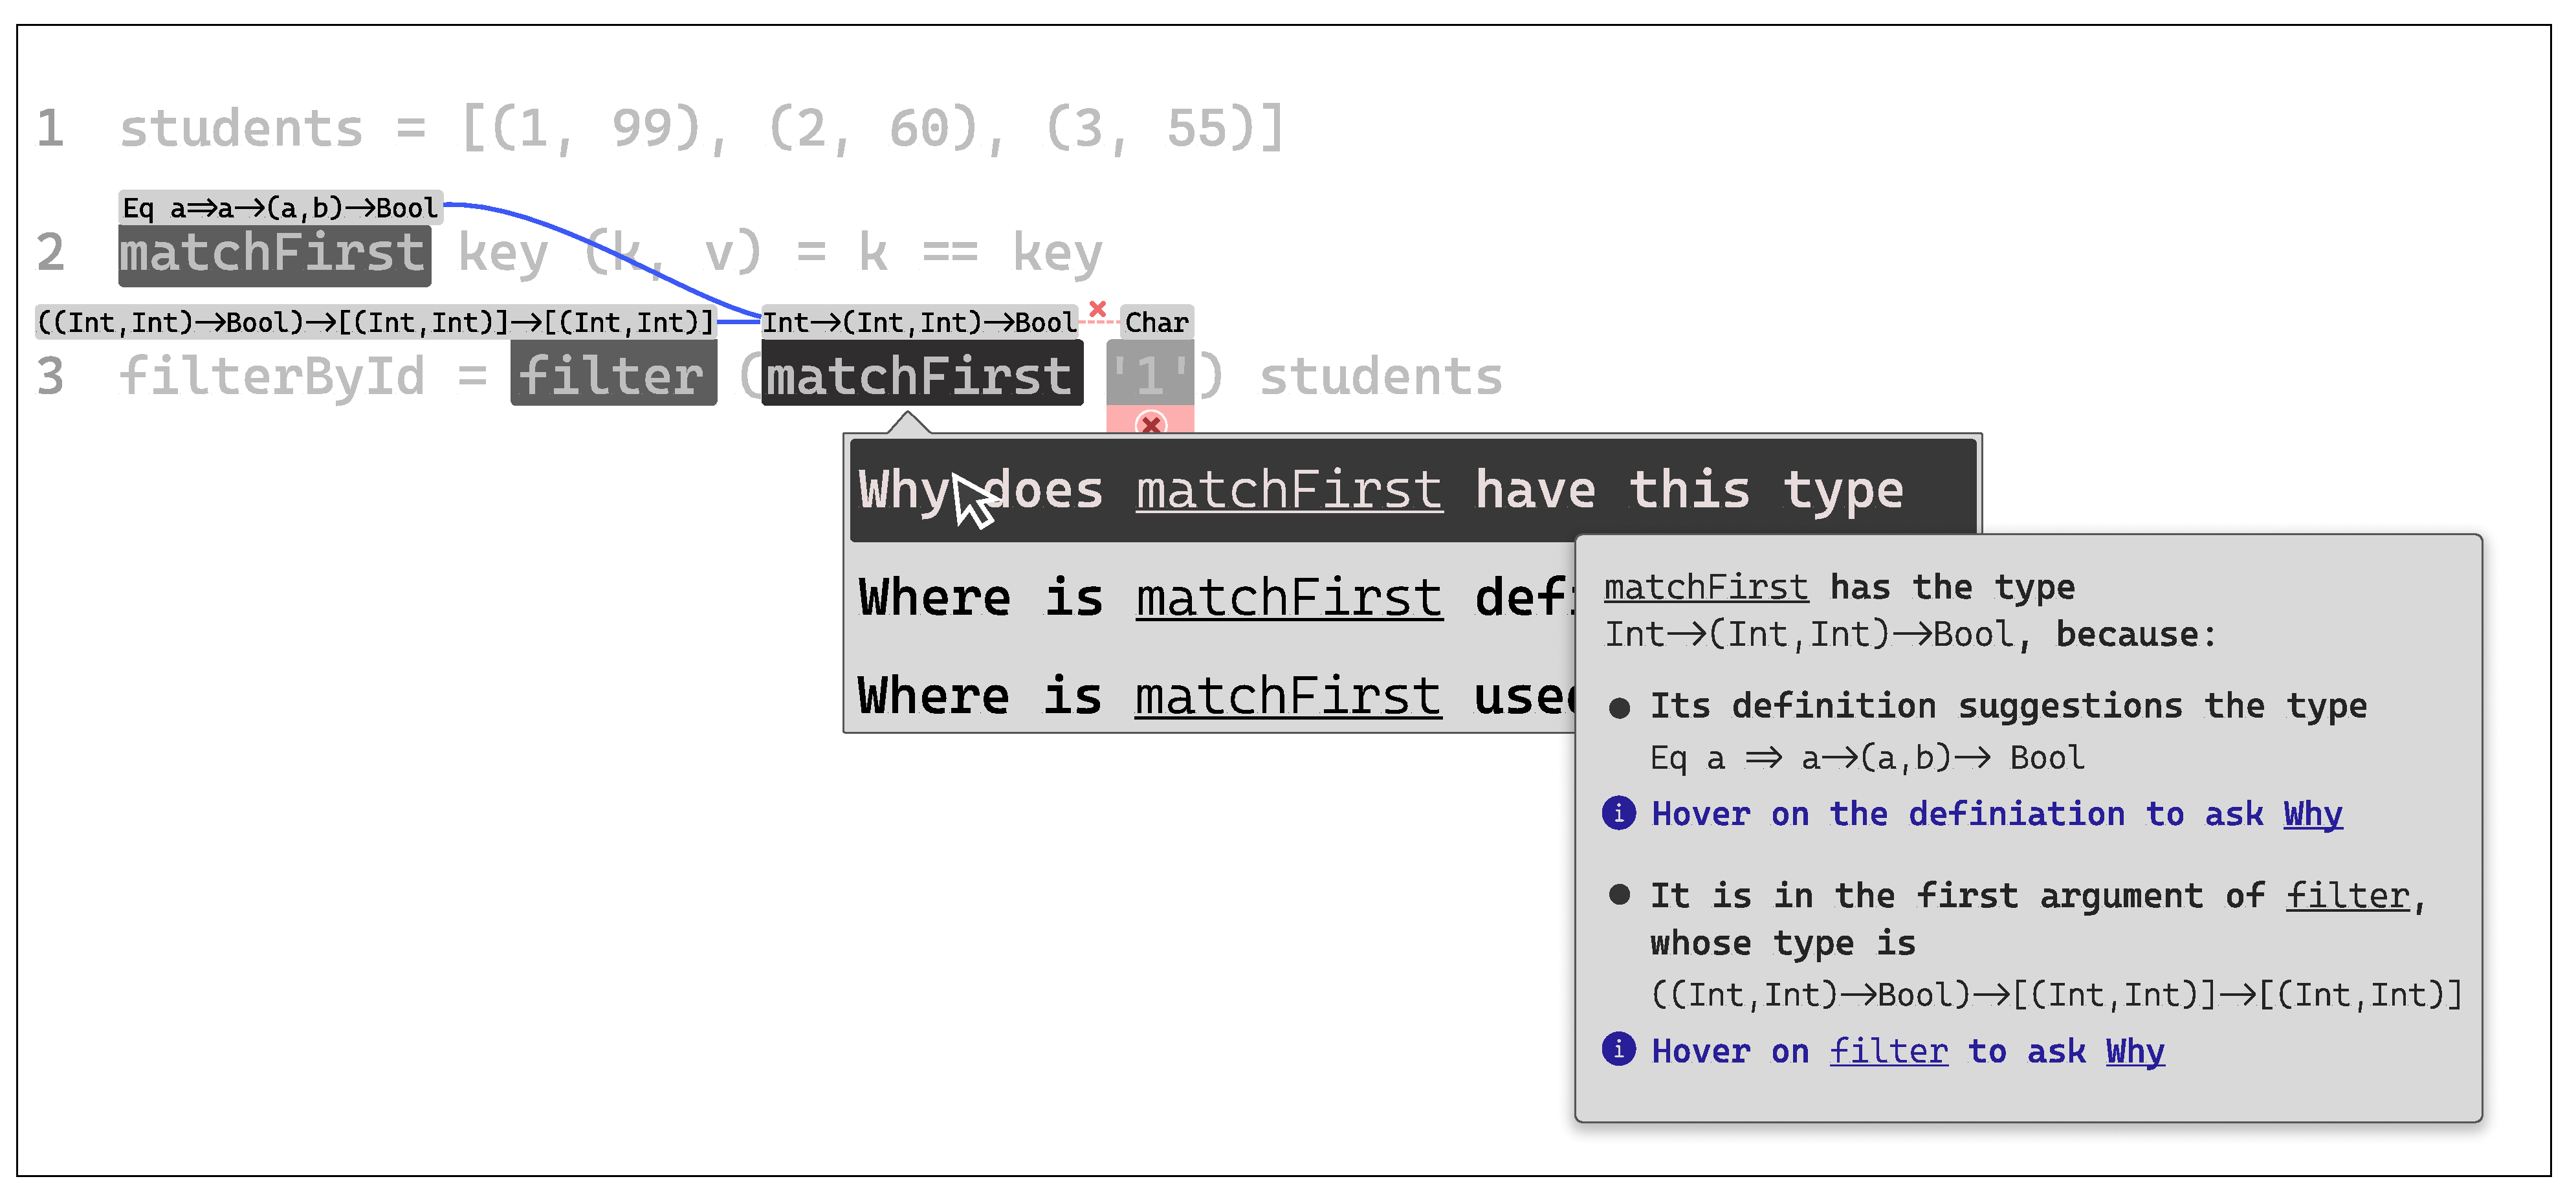
\includegraphics[width=\linewidth]{FollowUp}
  \caption[An example of \textit{TypeTutor} providing further explanation based on previous response (follow-up questions)]{
    \label{fig:follow-up}
     Following the case in Fig.~\ref{fig:why}, \textit{TypeTutor} will prompt programmers to ask follow-up questions. In this case, \textit{TypeTutor} will inform the programmer that \texttt{matchFirst} on line 3 has the type \texttt{Int -> (Int, Int) -> Bool} can be inferred from two pieces of clues:  the definition of \texttt{matchFirst} and the \texttt{filter} on line 3 instantiated as \texttt{((Int, Int) -> Bool) -> [(Int, Int)] -> [(Int, Int)]}. Programmers can trace further by following the hints again in the answer section.
    }
\end{figure}

\subsubsection*{How questions}

'How' questions in debugging focus on providing prescriptive guidance regarding program errors. Such questions do not solely depend on logical precision; they require understanding the knowledge gaps and delivering clear, followable instructions. \textit{TypeTutor} would aid programmers by facilitating questions on how to rectify specific type errors. In Goanna, the Maximal Satisfiable Subsets (MSS) analysis can suggest the recommended type for each possible correction. \textit{TypeTutor} would advance this concept by offering examples of syntax changes tailored to these recommended types. In the example (Fig.~\ref{fig:how}), \textit{TypeTutor} would provide various examples of how to change \texttt{'1'} to an Integer type, including changing it to an integer literal, an integer variable, or an expression that evaluates to an integer. 



\begin{figure}[hbt]
  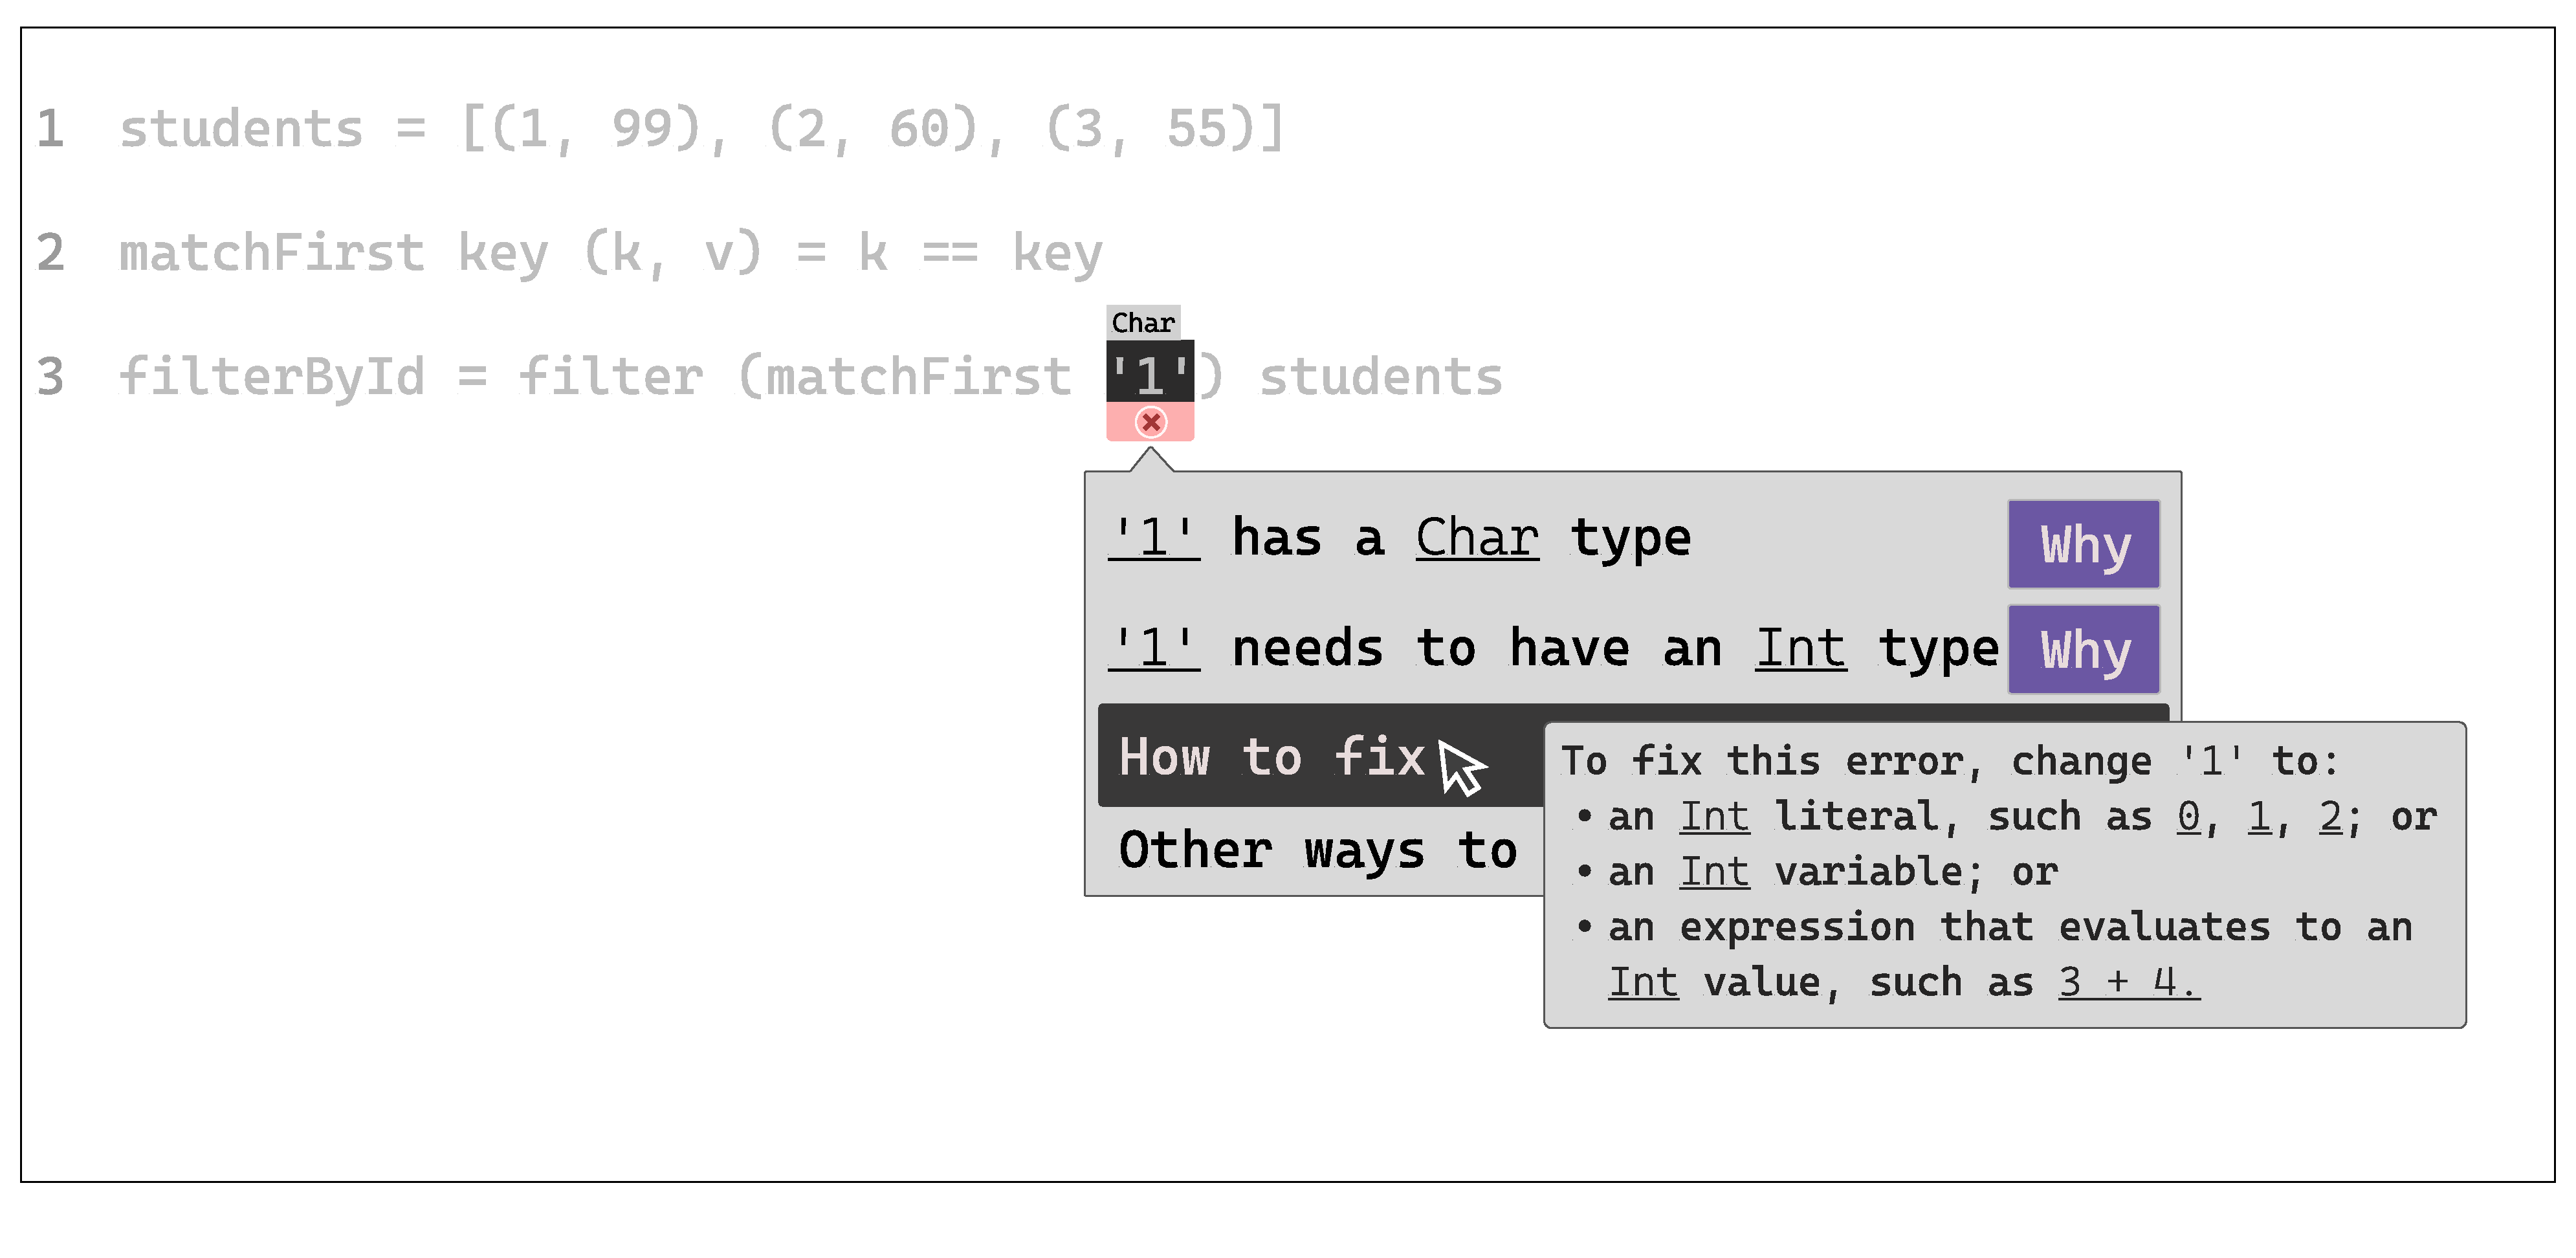
\includegraphics[width=\linewidth]{How}
  \caption[An example of \textit{TypeTutor} providing change suggestion (`how' questions)]{
    \label{fig:how}
    Following the case in Fig.~\ref{fig:why}, \textit{TypeTutor} will provide instructions on how to fix the type error. In detail,  \textit{TypeTutor} will provide various examples of how to change \texttt{'1'} to an Integer type, including changing it to an integer literal, an integer variable, or an expression that evaluates to an integer.
    }
\end{figure}

\subsubsection*{What-if questions}
Finally, as we have identified, type errors frequently involve multiple potential causes and explanations. When integrated into a question-and-answer interface, the presence of multiple causes naturally prompts counterfactual questions such as "What are other ways that can cause this type error?" Recognizing this, \textit{TypeTutor} will provide a natural and user-friendly interface for exploring various potential causes and solutions. This approach, while similar to the functionality offered by Goanna, features a more concise and intuitive interface for programmers to switch between different potential causes. With \textit{TypeTutor}, programmers will find the option: `Other ways to fix the error' in every type error question list; hovering over the option will present alternative explanations and resolution plans (Fig.~\ref{fig:what-if}).

\begin{figure}[hbt]
  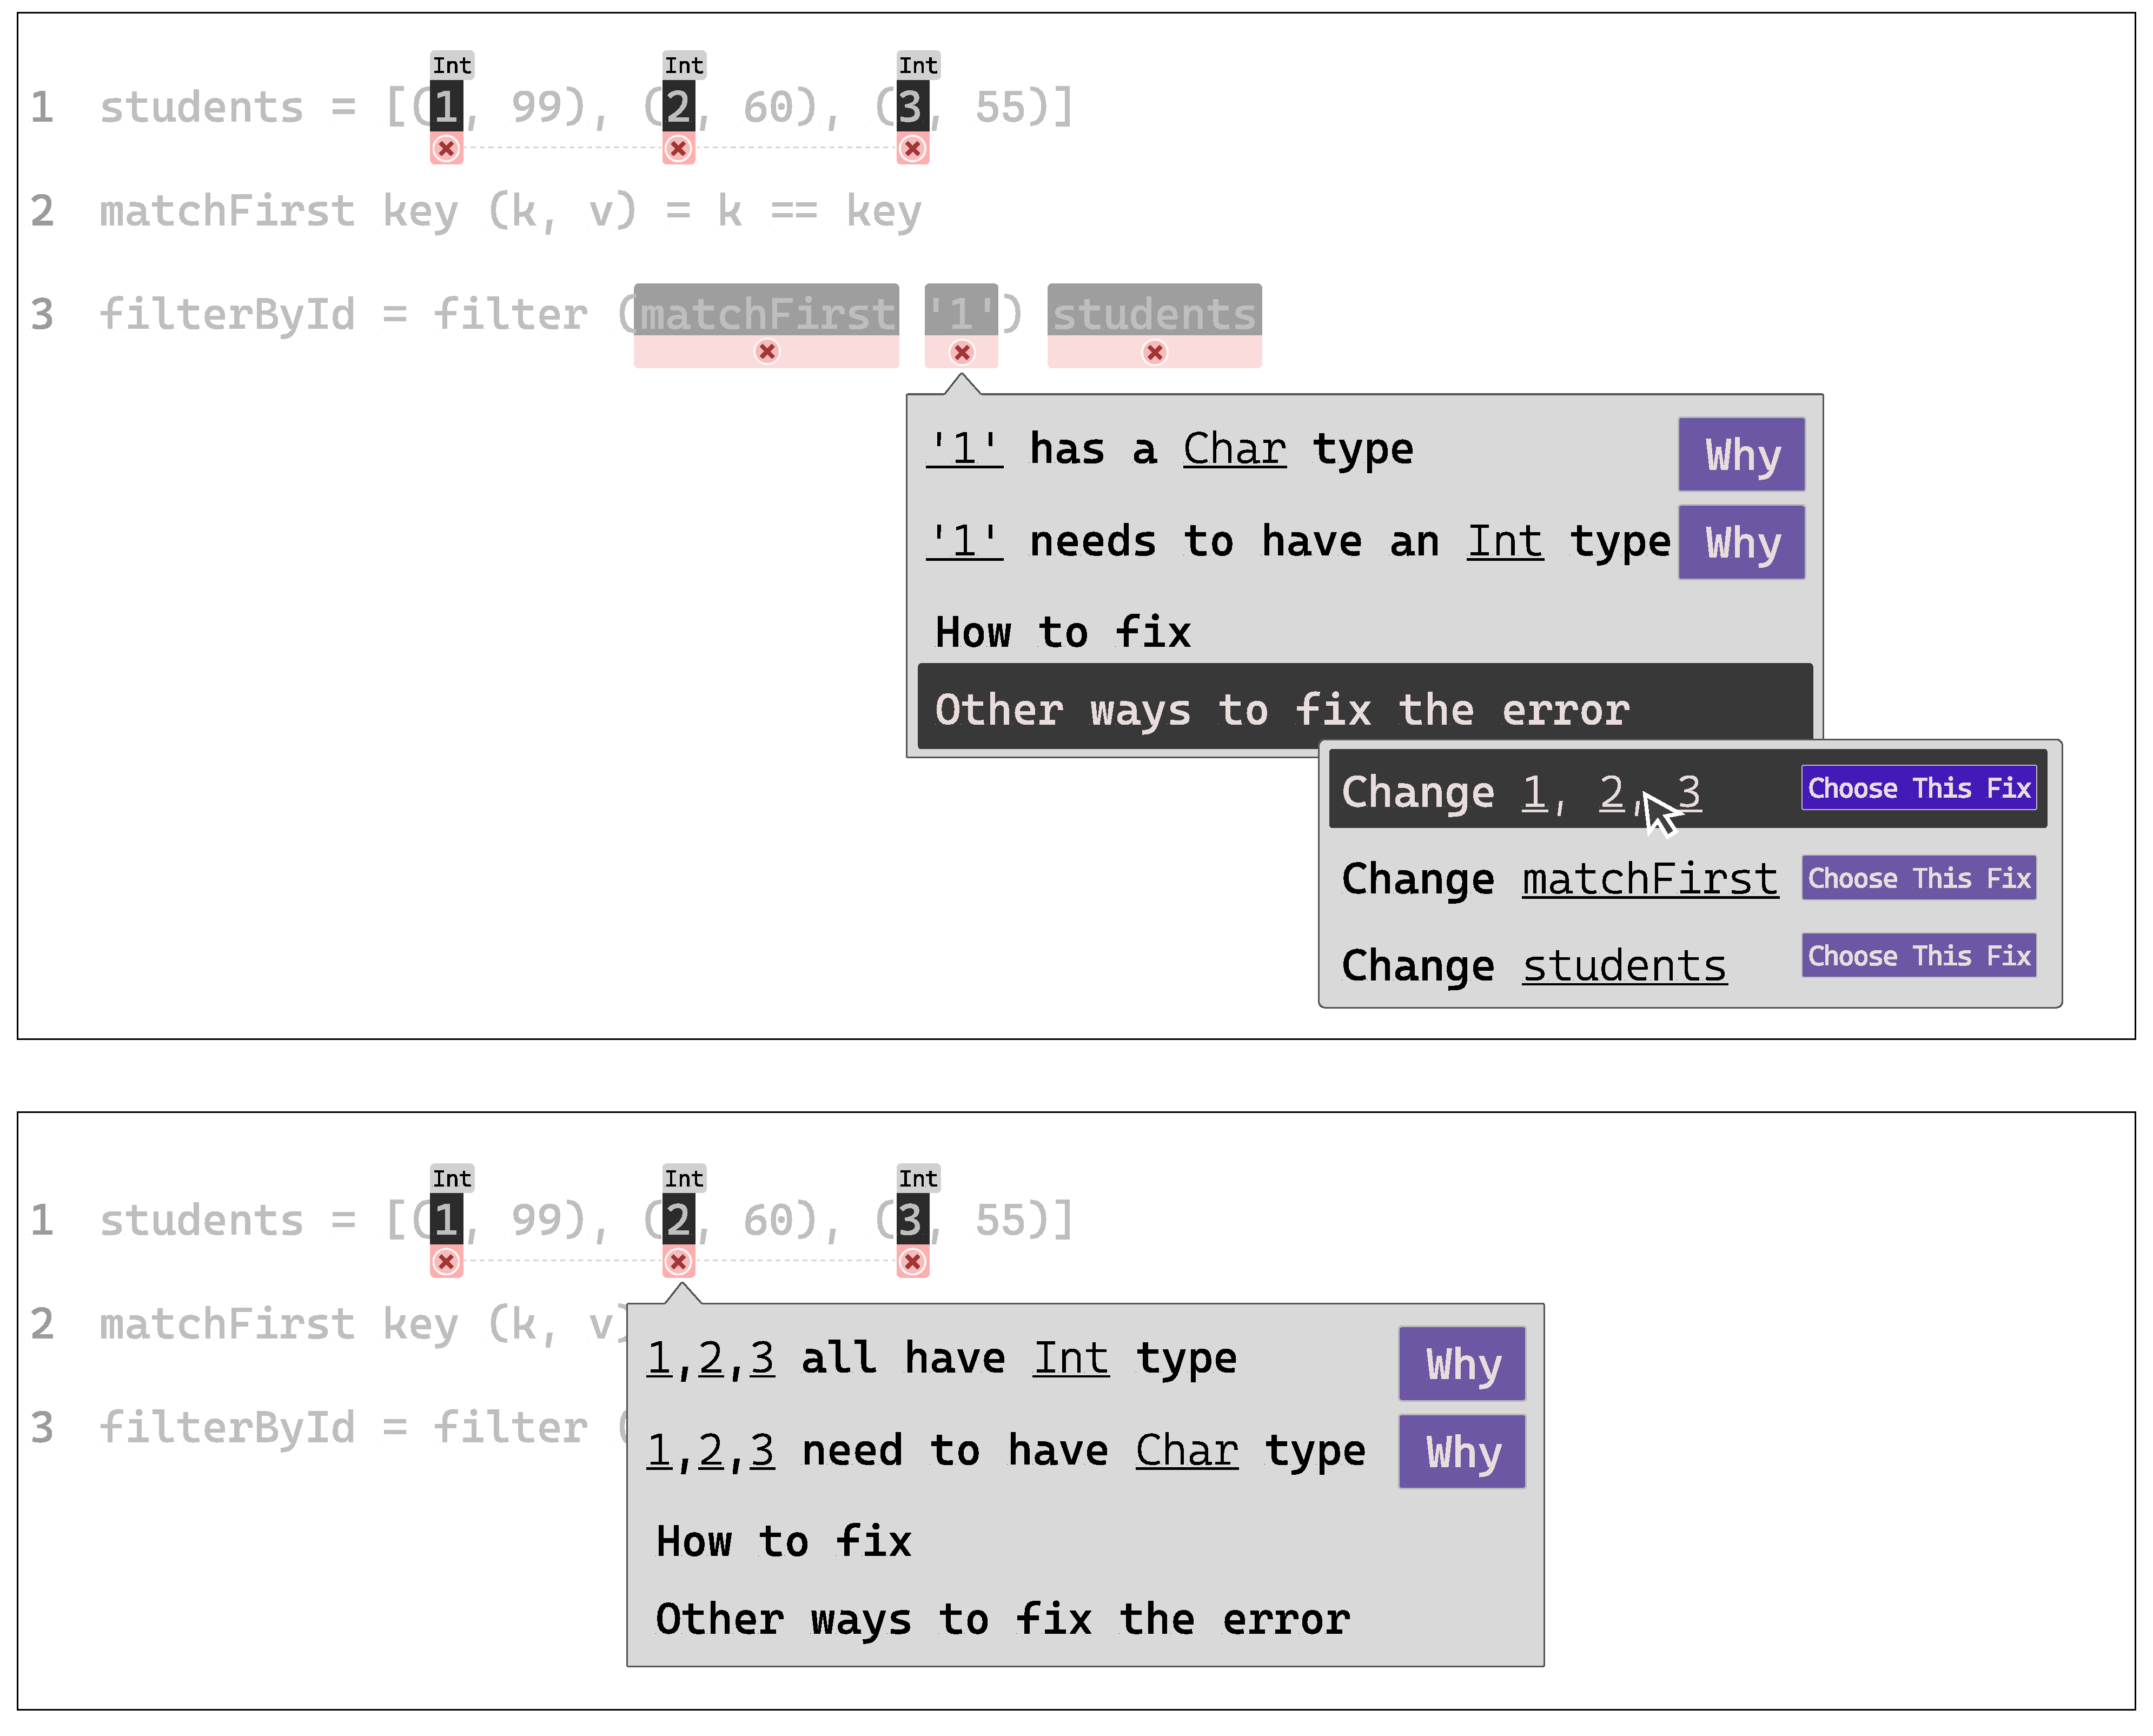
\includegraphics[width=\linewidth]{WhatIf}
  \caption[An examples of \textit{TypeTutor} addressing alternative causes (`what-if' questions)]{
      \label{fig:what-if}
      If the programmer disagrees that the literal \texttt{'1'} is the cause of the error and should be changed, \textit{TypeTutor} will provide alternative explanations and resolution plans. When hovering on the option `Other ways to fix the error', \textit{TypeTutor} will show three other potential fixes (Top). Choosing any of them, say the first option, will change the type error mark to another set of locations, and different explanations are provided when asking the `why' question at the new type error.
    }
\end{figure}


\subsection*{Integration with Large Language Models}
At the time of writing this thesis, LLMs were actively experimented with performing all kinds of tasks that require human creativity, including programming. Many attempts have been made to use LLMs in programming tasks \cite{Shi2024-bj}, intending to free programmers for higher-level thinking. This development is tangential to our objective of explaining type errors and reasoning about the logic of type inference. 

\begin{figure}[hbt]
  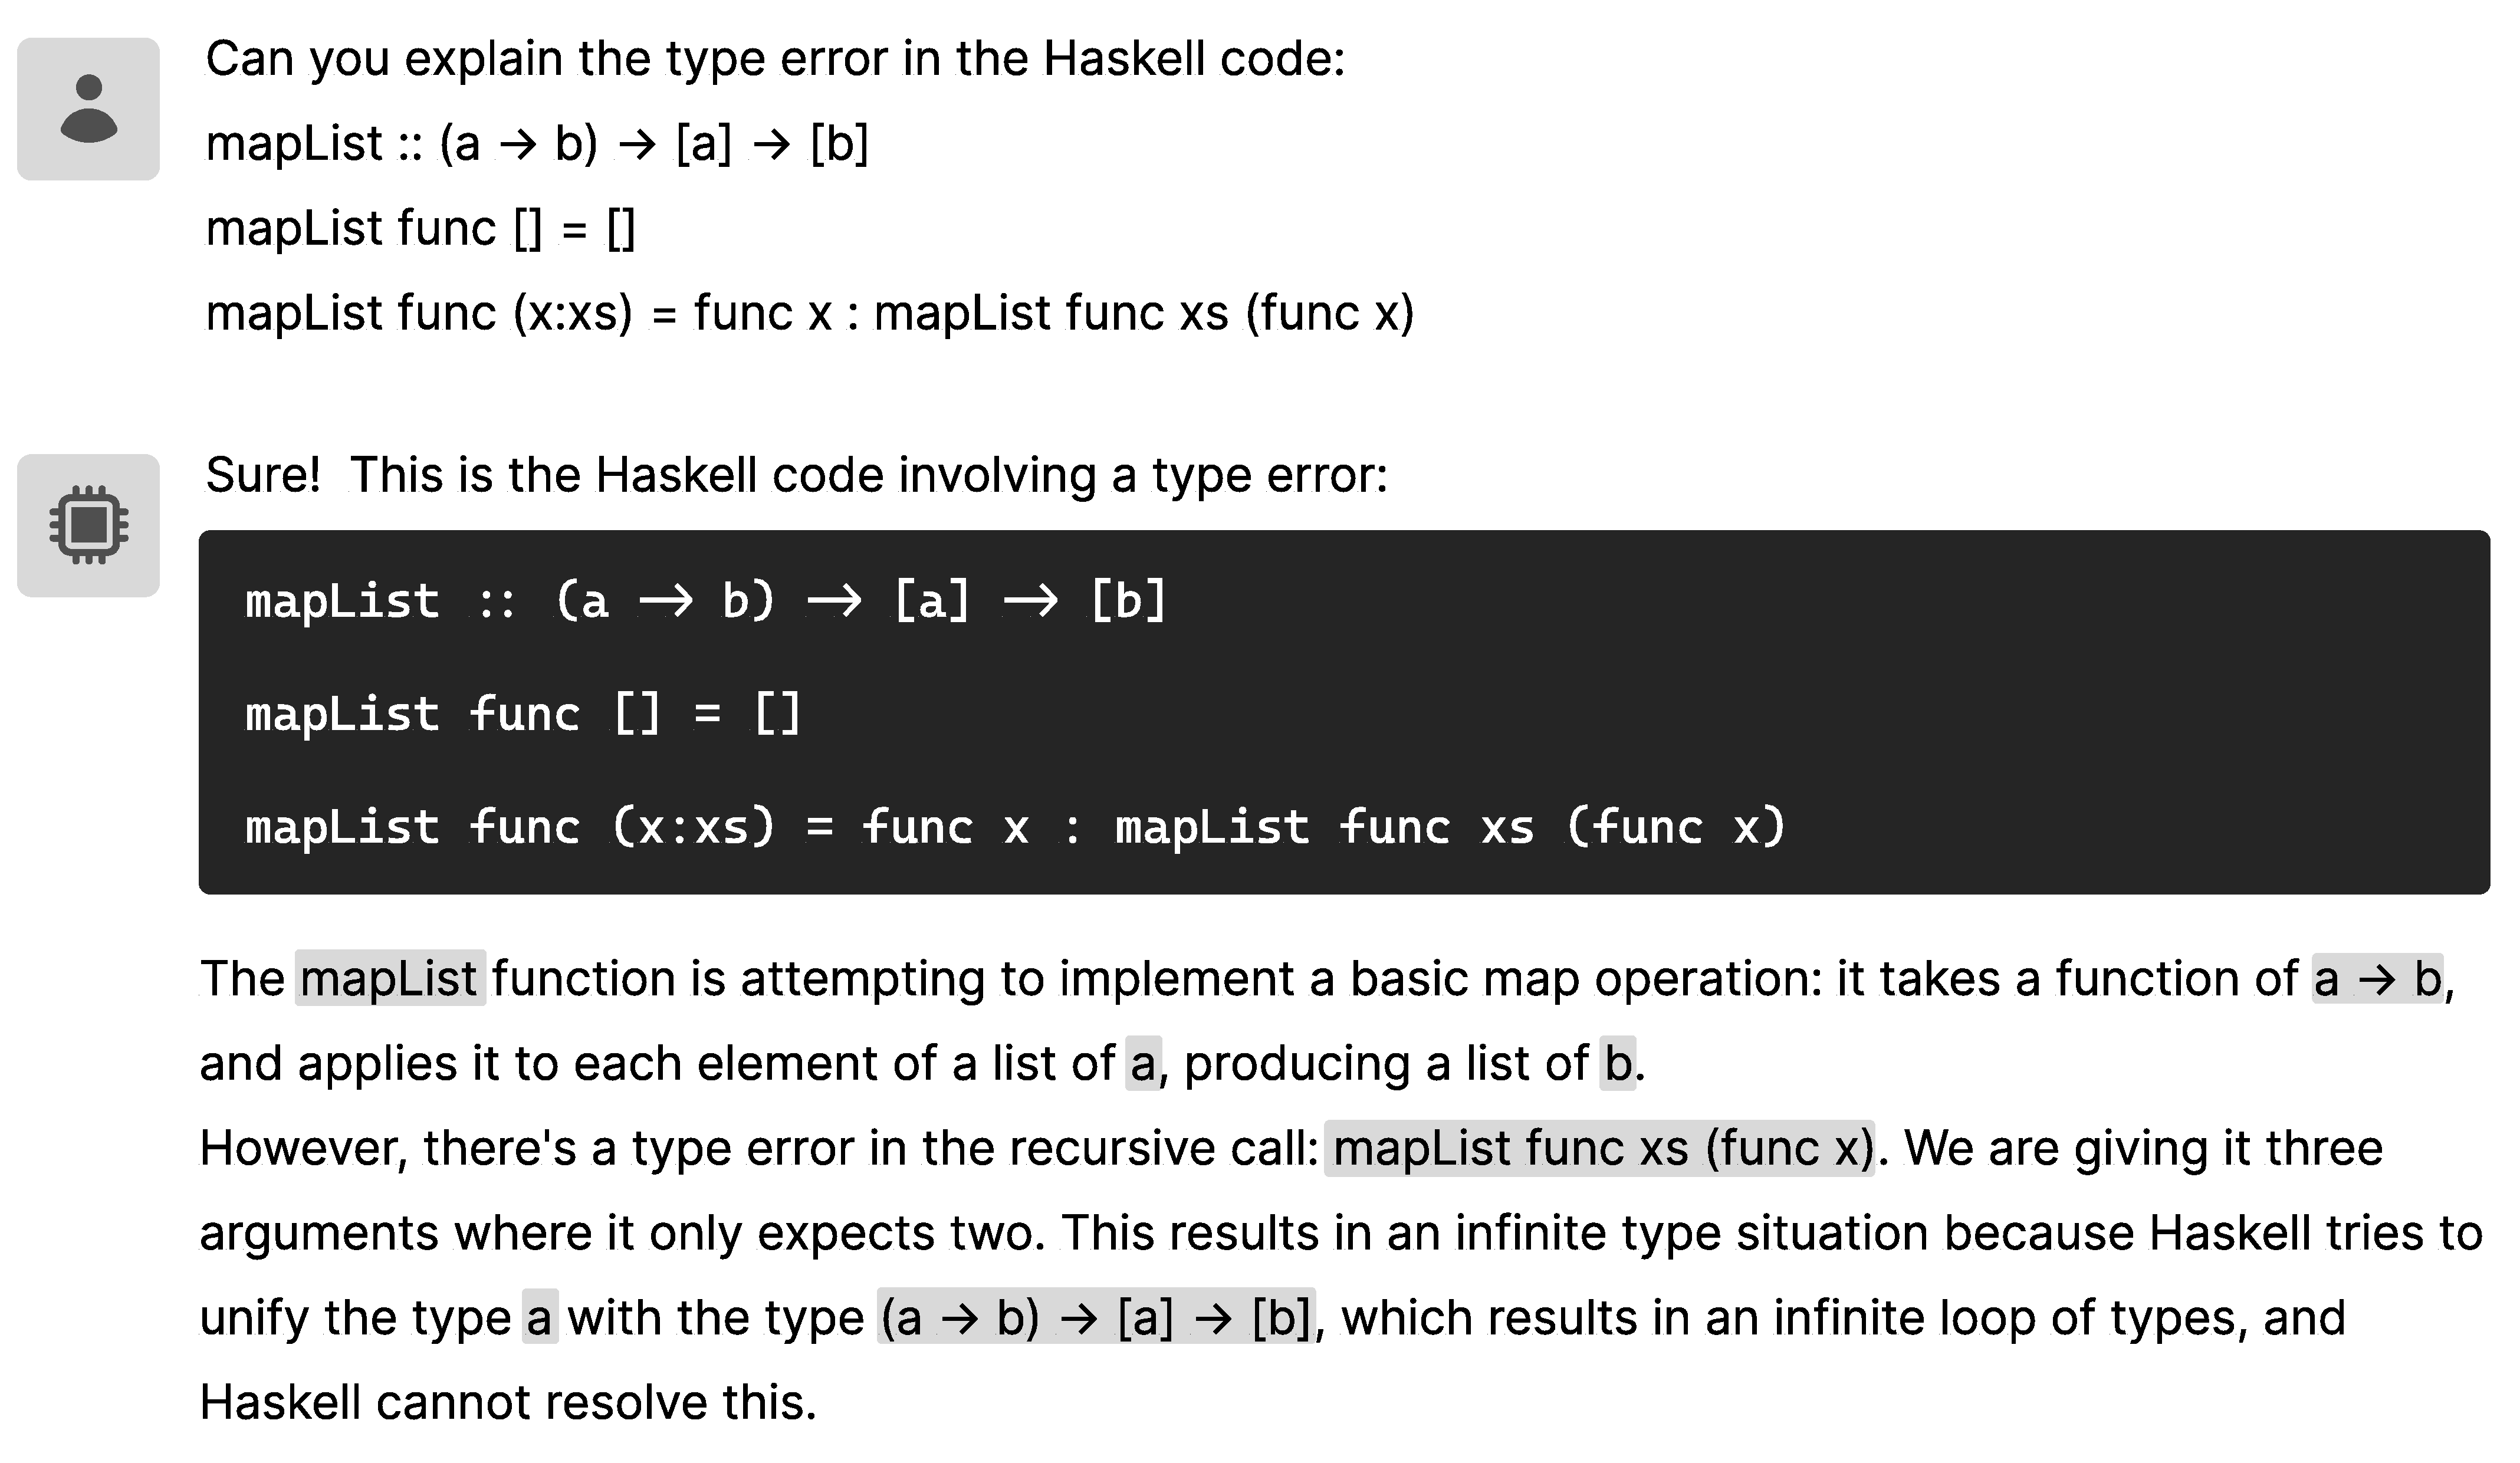
\includegraphics[width=\linewidth]{LLM}
  \caption[LLM explaining a type error; it began very accurate, then went on to give incorrect and contradicting analysis]{\label{fig:llm}
  The figure shows the user prompted LLM to explain the type error in a Haskell function definition \texttt{mapList}. LLM, at first, showed a profound understanding of the subject matter, clearly explained the intention of the function, and accurately identified the error location. In the last sentence, LLM claimed the definition would result in an infinite type because trying to unify \texttt{a} with \texttt{(a -> b) -> [a] -> [b]}. In reality, unifying two functions with different numbers of arguments will not cause infinite types. 
    }
\end{figure}

While LLMs have shown capability in recognizing basic errors, they often display a limited understanding of type theories and multi-step reasoning ability. Fig.~\ref{fig:llm} depicts a type error caused by mismatching numbers of arguments in the function \texttt{mapList}; although provided a correct error identification at the start, GPT 4 proceeded to claim, “This results in an infinite type situation because Haskell tries to unify the type \texttt{a} with the type \texttt{(a -> b) -> [a] -> [b]}, which results in an infinite loop of types, and Haskell cannot resolve this,” illustrating a fundamental lack of understanding of type theory.

\begin{figure}[hbt]
  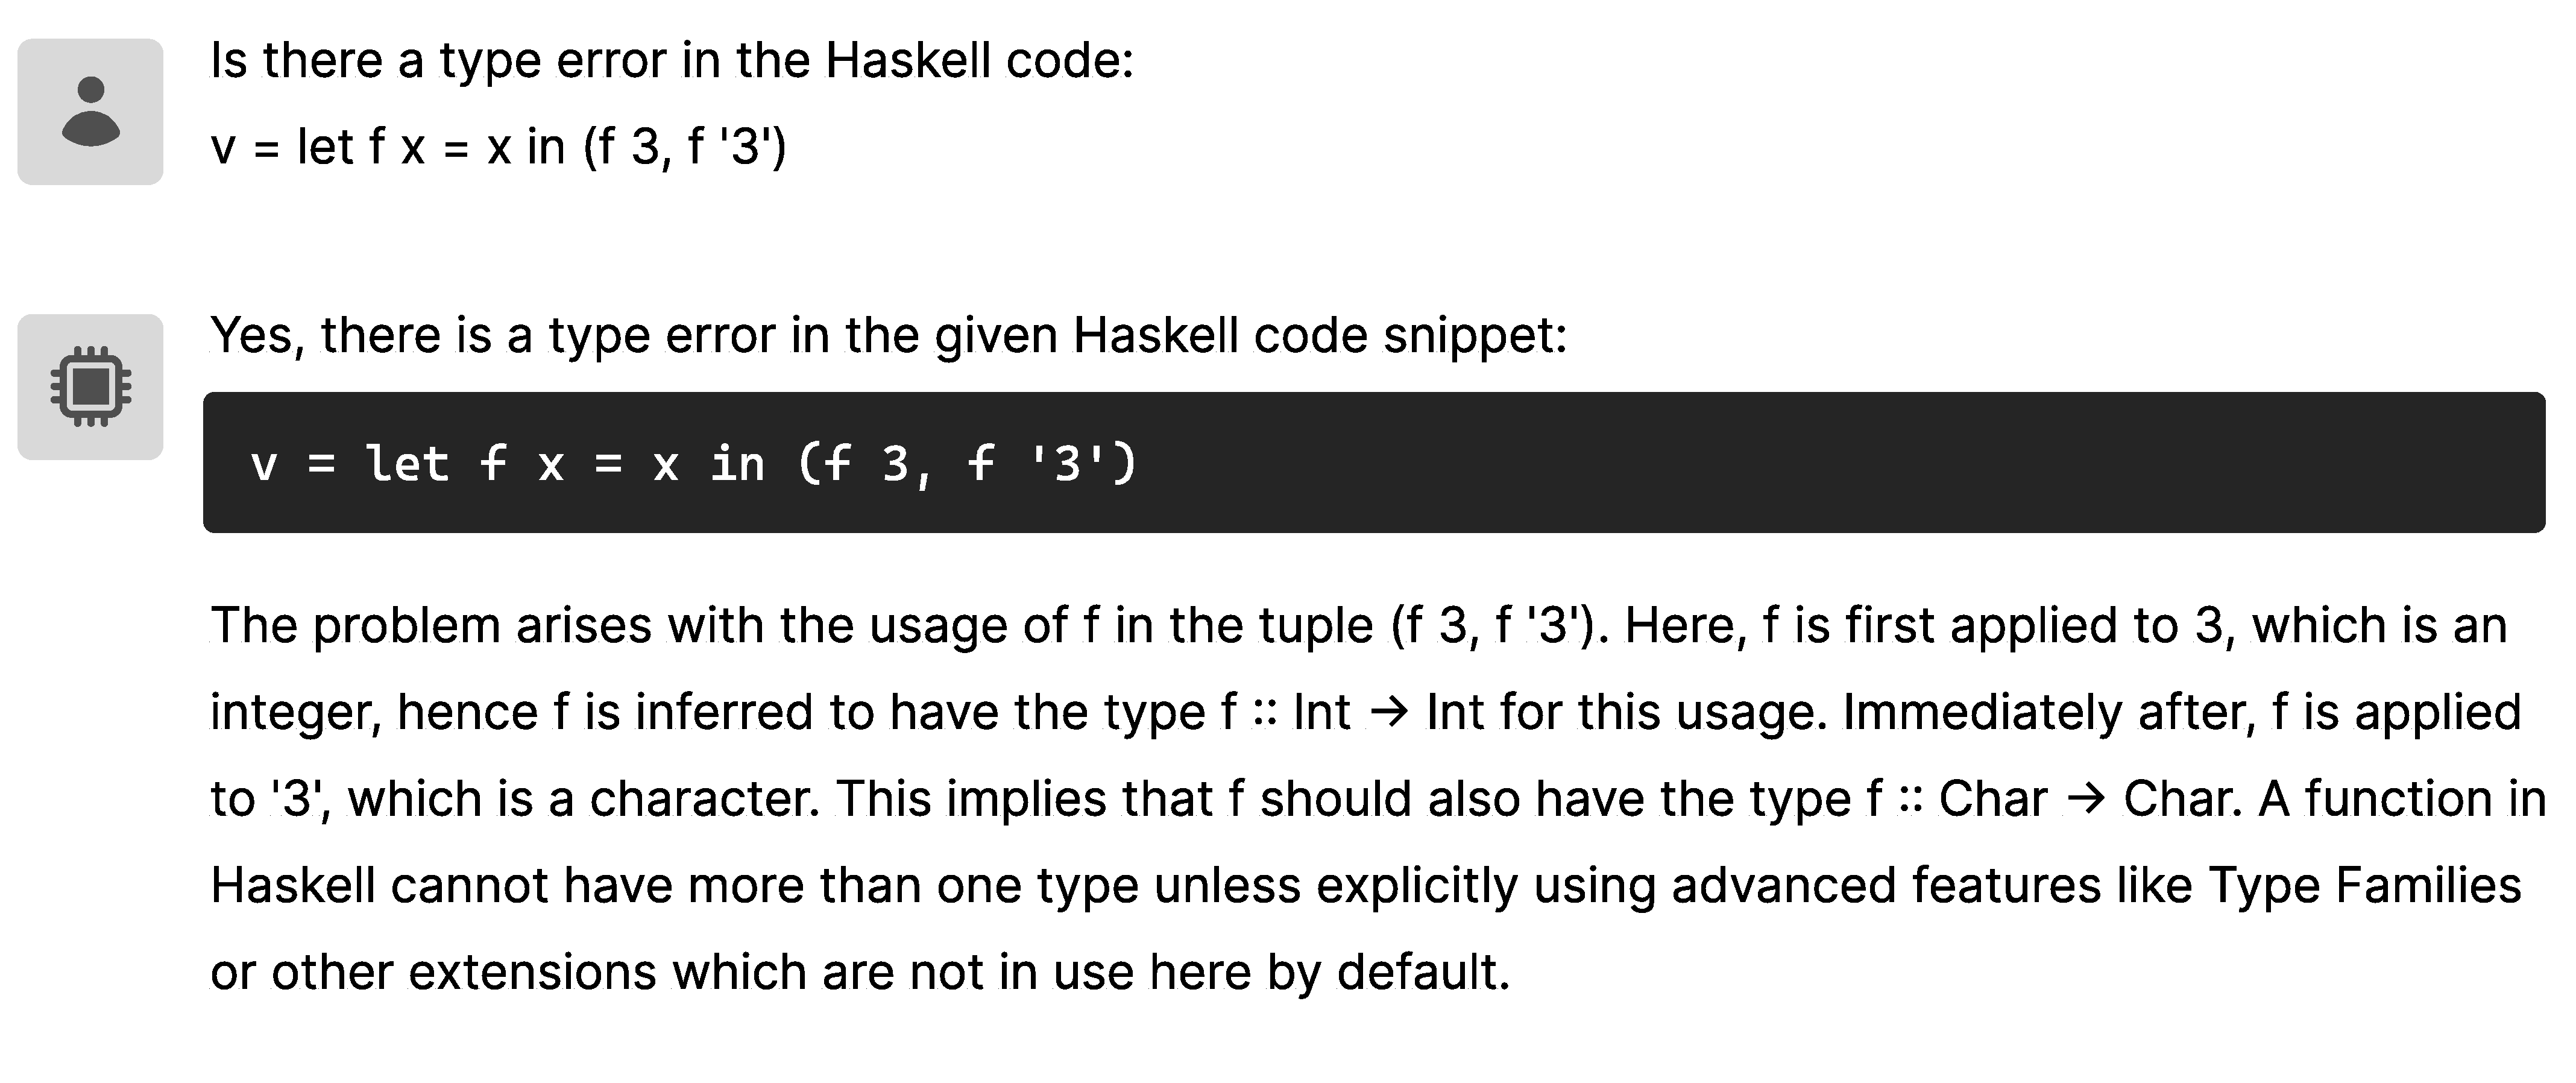
\includegraphics[width=\linewidth]{LLM2}
  \caption[An example where LLM identified a type error in well-typed source code]{\label{fig:llm2}
  The figure shows a user asking an LLM whether the provided Haskell source code has a type error. While the provided code is, in fact, well-typed, LLM hallucinated a type error and ignored how polymorphic functions work in Haskell. In the example, the function \texttt{f},  defined the same way as the \texttt{id} function, can be applied with a value of any type.
    } 
\end{figure}

When tested with the prompt "Is there a type error in the Haskell code: v = let f x = x in (f 3, f '3')", most LLMs incorrectly reported yes (Fig.~\ref{fig:llm2}). However, this Haskell code is indeed well-typed. LLMs can give wrong explanations and find type errors that do not exist, unlike tools like GHC, Helium, and Goanna. While there is clearly a role for their usage in programming assistance \cite{Lee2024-hs}, they do not “reason” about types and, hence, are not trustworthy.

While LLMs are getting more and more accurate with each iteration, some doubt whether they will ever become as reliable as theory-based tools \cite{Berglund2023-ig}. We believe in the great potential of integrating LLMs with existing theory-based tools, such as \chameleon{} and Goanna. This integration could enhance the performance of LLMs by aligning their operations with accurate theoretical guides or utilizing their strengths in areas where traditional tools fall short, such as suggesting syntactical improvements. This synergy could lead to more robust programming assistance using both types of tools. We propose two candidate workflows:

\itemize{
  \item{\textbf{Code Generation and Validation}: LLMs could generate initial source code based on user-provided prompts. Theory-based tools, such as \chameleon{} and Goanna, then check for errors. Detected errors could be fed back to the LLMs for corrections, enhancing both the efficiency and accuracy of code development.}
  \item {\textbf{Error Tutoring and Resolution}: Theory-based tools could identify errors in manually written code, with LLMs suggesting syntax corrections. This combines the precise error detection from traditional theory-based tools with the ability of LLMs to generate effective syntax changes, surpassing traditional tools in this domain.}
}

\subsection*{Support for Other Languages}
Haskell serves as a vital platform for the experiments of programming languages and type systems. We firmly believe that the next critical phase in our research involves expanding our tools to encompass other languages. Recently, we observed that the challenges of overcoming complex type errors have permeated several mainstream languages, including Rust \cite{Zeng2019-ou} and TypeScript \cite{Scarsbrook2023-uq}. By integrating our debugging tools into these languages, we would be able to engage a broader audience and subject our tools to a diverse range of software projects varying in style and scale. This will not only increase the applicability of our tools but also provide us with extensive insights into how to further improve our design.

Much of our work has already been conceived with the adaptability to multiple languages in mind. For example, GeckoGraph is designed to be language-agnostic, allowing for implementations in different programming languages. However, adapting tools like \chameleon{} and Goanna presents certain complexities. Although the analysis of unsatisfiable constraints and the theories and implementations concerning the enumeration of Minimal Unsatisfiable Subsets (MUSes) and Minimal Correction Subsets (MCSes) are universally applicable across all languages, specific challenges arise when taking into account the nuances of individual languages.

The first challenge involves constraint generation. Each language requires the development of specific rules for generating constraints and conforming to its own typing rules, which could necessitate substantial modifications depending on the type-level features each language possesses. For instance, all functions in Haskell are curried, meaning that they can be provided with fewer arguments than they are defined, a characteristic absent in TypeScript, where functions are defined with fixed arity and can be overloaded. This discrepancy means that in TypeScript, a type error can occur if a function is applied to fewer arguments than it is defined for, an error that would not typically arise in Haskell.

The second challenge concerns the presentation of type errors, which may need nuanced adjustments for different languages. For example, novel visualization techniques may be required to effectively convey concepts absent in Haskell, such as row polymorphism in TypeScript or lifetime constraints in Rust. By addressing these challenges, we can truly leverage the potential of our tools across various programming environments.

\subsubsection*{Supporting Dependently Typed Languages}

As mentioned in previous chapters, dependently typed languages like Idris and Agda represent a rigorous subclass within the realm of statically typed languages. These languages uniquely enable the type-level computation of values and types, allowing programmers to embed fine-grained and precise constraints to ensure program correctness at compile time. Due to their ability to directly encode program behavior into types, programs written in dependently typed languages can often be validated purely through the type-checking process. This makes them ideal candidates for code generation through LLMs, where programmers can perform checks on whether they conform to the provided specifications. 

However, despite their potential, dependently typed languages currently hold a modest position in the mainstream programming landscape. We believe that enhancing our type debugging tools to support dependently typed languages can bring a step forward in improving their learnability and adoption, especially among programmers who are new to dependent typing. As type-level computations grow in complexity, our tools, designed to aid in understanding and reasoning, become increasingly valuable. 


\section{Conclusion}


The field of programming languages is truly captivating, representing a confluence of ideas from various disciplines and schools of thought. Among the myriad concepts, functional programming and static typing are particularly important for their profound impact on the domain. My research aims to highlight the benefits of functional programming and static typing while also addressing the challenges they pose. By refining how types and type errors are presented and explained, we strive to make functional programming and static typing accessible and user-friendly to programmers.

Our methodologies are largely grounded in theories of constraint satisfiability. These include analyzing Minimal Unsatisfiable Subsets (MUS) through tools like \chameleon{} and Minimal Correction Subsets (MCS) via Goanna. In addition, we employ various human-centered research techniques, such as formative studies, user studies, and rapid prototyping. These approaches enhance the practicality of our research and, hopefully, its relevance to real-world programming.

We are convinced that type error enhancement and explanation is a valuable trajectory for research in programming languages. It is our hope that our work will serve as a helpful reference, inspiring future studies that continue to augment and expand our arsenal of type error debugging tools.


